\documentclass[twoside]{book}

% Packages required by doxygen
\usepackage{fixltx2e}
\usepackage{calc}
\usepackage{doxygen}
\usepackage[export]{adjustbox} % also loads graphicx
\usepackage{graphicx}
\usepackage[utf8]{inputenc}
\usepackage{makeidx}
\usepackage{multicol}
\usepackage{multirow}
\PassOptionsToPackage{warn}{textcomp}
\usepackage{textcomp}
\usepackage[nointegrals]{wasysym}
\usepackage[table]{xcolor}

% Font selection
\usepackage[T1]{fontenc}
\usepackage[scaled=.90]{helvet}
\usepackage{courier}
\usepackage{amssymb}
\usepackage{sectsty}
\renewcommand{\familydefault}{\sfdefault}
\allsectionsfont{%
  \fontseries{bc}\selectfont%
  \color{darkgray}%
}
\renewcommand{\DoxyLabelFont}{%
  \fontseries{bc}\selectfont%
  \color{darkgray}%
}
\newcommand{\+}{\discretionary{\mbox{\scriptsize$\hookleftarrow$}}{}{}}

% Page & text layout
\usepackage{geometry}
\geometry{%
  a4paper,%
  top=2.5cm,%
  bottom=2.5cm,%
  left=2.5cm,%
  right=2.5cm%
}
\tolerance=750
\hfuzz=15pt
\hbadness=750
\setlength{\emergencystretch}{15pt}
\setlength{\parindent}{0cm}
\setlength{\parskip}{3ex plus 2ex minus 2ex}
\makeatletter
\renewcommand{\paragraph}{%
  \@startsection{paragraph}{4}{0ex}{-1.0ex}{1.0ex}{%
    \normalfont\normalsize\bfseries\SS@parafont%
  }%
}
\renewcommand{\subparagraph}{%
  \@startsection{subparagraph}{5}{0ex}{-1.0ex}{1.0ex}{%
    \normalfont\normalsize\bfseries\SS@subparafont%
  }%
}
\makeatother

% Headers & footers
\usepackage{fancyhdr}
\pagestyle{fancyplain}
\fancyhead[LE]{\fancyplain{}{\bfseries\thepage}}
\fancyhead[CE]{\fancyplain{}{}}
\fancyhead[RE]{\fancyplain{}{\bfseries\leftmark}}
\fancyhead[LO]{\fancyplain{}{\bfseries\rightmark}}
\fancyhead[CO]{\fancyplain{}{}}
\fancyhead[RO]{\fancyplain{}{\bfseries\thepage}}
\fancyfoot[LE]{\fancyplain{}{}}
\fancyfoot[CE]{\fancyplain{}{}}
\fancyfoot[RE]{\fancyplain{}{\bfseries\scriptsize Generated by Doxygen }}
\fancyfoot[LO]{\fancyplain{}{\bfseries\scriptsize Generated by Doxygen }}
\fancyfoot[CO]{\fancyplain{}{}}
\fancyfoot[RO]{\fancyplain{}{}}
\renewcommand{\footrulewidth}{0.4pt}
\renewcommand{\chaptermark}[1]{%
  \markboth{#1}{}%
}
\renewcommand{\sectionmark}[1]{%
  \markright{\thesection\ #1}%
}

% Indices & bibliography
\usepackage{natbib}
\usepackage[titles]{tocloft}
\setcounter{tocdepth}{3}
\setcounter{secnumdepth}{5}
\makeindex

% Hyperlinks (required, but should be loaded last)
\usepackage{ifpdf}
\ifpdf
  \usepackage[pdftex,pagebackref=true]{hyperref}
\else
  \usepackage[ps2pdf,pagebackref=true]{hyperref}
\fi
\hypersetup{%
  colorlinks=true,%
  linkcolor=blue,%
  citecolor=blue,%
  unicode%
}

% Custom commands
\newcommand{\clearemptydoublepage}{%
  \newpage{\pagestyle{empty}\cleardoublepage}%
}

\usepackage{caption}
\captionsetup{labelsep=space,justification=centering,font={bf},singlelinecheck=off,skip=4pt,position=top}

%===== C O N T E N T S =====

\begin{document}

% Titlepage & ToC
\hypersetup{pageanchor=false,
             bookmarksnumbered=true,
             pdfencoding=unicode
            }
\pagenumbering{roman}
\begin{titlepage}
\vspace*{7cm}
\begin{center}%
{\Large Matrix Operations }\\
\vspace*{1cm}
{\large Generated by Doxygen 1.8.11}\\
\end{center}
\end{titlepage}
\clearemptydoublepage
\tableofcontents
\clearemptydoublepage
\pagenumbering{arabic}
\hypersetup{pageanchor=true}

%--- Begin generated contents ---
\chapter{Class Index}
\section{Class List}
Here are the classes, structs, unions and interfaces with brief descriptions\+:\begin{DoxyCompactList}
\item\contentsline{section}{\hyperlink{classMatrix}{Matrix$<$ T, m, n $>$} \\*Class used for member function definitions. Uses templates }{\pageref{classMatrix}}{}
\end{DoxyCompactList}

\chapter{File Index}
\section{File List}
Here is a list of all documented files with brief descriptions\+:\begin{DoxyCompactList}
\item\contentsline{section}{/home/sudartion/cpp\+\_\+ws/matrix\+\_\+operations/include/{\bfseries matrix\+\_\+functions.\+hpp} }{\pageref{matrix__functions_8hpp}}{}
\item\contentsline{section}{/home/sudartion/cpp\+\_\+ws/matrix\+\_\+operations/src/\hyperlink{demo_8cpp}{demo.\+cpp} \\*\hyperlink{classMatrix}{Matrix} operations definition }{\pageref{demo_8cpp}}{}
\item\contentsline{section}{/home/sudartion/cpp\+\_\+ws/matrix\+\_\+operations/test/\hyperlink{main_8cpp}{main.\+cpp} \\*Test cases for code coverage }{\pageref{main_8cpp}}{}
\item\contentsline{section}{/home/sudartion/cpp\+\_\+ws/matrix\+\_\+operations/test/\hyperlink{test_8cpp}{test.\+cpp} \\*\hyperlink{classMatrix}{Matrix} operations definition }{\pageref{test_8cpp}}{}
\end{DoxyCompactList}

\chapter{Class Documentation}
\hypertarget{classMatrix}{}\section{Matrix$<$ T, m, n $>$ Class Template Reference}
\label{classMatrix}\index{Matrix$<$ T, m, n $>$@{Matrix$<$ T, m, n $>$}}


Class used for member function definitions. Uses templates.  




{\ttfamily \#include $<$matrix\+\_\+functions.\+hpp$>$}

\subsection*{Public Member Functions}
\begin{DoxyCompactItemize}
\item 
\hyperlink{classMatrix_a48672cd6372a2bd80816321c0ffb8757}{Matrix} (vector$<$ vector$<$ T $>$ $>$ \&a)
\begin{DoxyCompactList}\small\item\em Constructor of class. Used to create matrix. \end{DoxyCompactList}\item 
\hyperlink{classMatrix_a0fc90e09b1eddc059e70881ad8f17ba2}{$\sim$\+Matrix} ()\hypertarget{classMatrix_a0fc90e09b1eddc059e70881ad8f17ba2}{}\label{classMatrix_a0fc90e09b1eddc059e70881ad8f17ba2}

\begin{DoxyCompactList}\small\item\em Destructor. \end{DoxyCompactList}\item 
void \hyperlink{classMatrix_ac161952679186c23c5785e5bcfef2cb7}{print} ()
\begin{DoxyCompactList}\small\item\em Function to print out the matrix and display. \end{DoxyCompactList}\item 
\hyperlink{classMatrix}{Matrix}$<$ T, n, m $>$ \hyperlink{classMatrix_a99567eedc9e9213b2047352e01f1abb4}{transpose} ()
\begin{DoxyCompactList}\small\item\em Function to create transpose. \end{DoxyCompactList}\end{DoxyCompactItemize}
\subsection*{Public Attributes}
\begin{DoxyCompactItemize}
\item 
int {\bfseries nrow}\hypertarget{classMatrix_abf937e657da2a3a625f704fd1568a9b0}{}\label{classMatrix_abf937e657da2a3a625f704fd1568a9b0}

\item 
int {\bfseries ncol}\hypertarget{classMatrix_a487a37e9cff00849712b7f7518fcd669}{}\label{classMatrix_a487a37e9cff00849712b7f7518fcd669}

\item 
bool {\bfseries flag1}\hypertarget{classMatrix_a5f7fde3d29abf2546c0a493492aa493d}{}\label{classMatrix_a5f7fde3d29abf2546c0a493492aa493d}

\item 
bool {\bfseries flag2}\hypertarget{classMatrix_a7980c98c92fa7235fa622714281deda7}{}\label{classMatrix_a7980c98c92fa7235fa622714281deda7}

\end{DoxyCompactItemize}
\subsection*{Friends}
\begin{DoxyCompactItemize}
\item 
class {\bfseries Matrix$<$ T, n, m $>$}\hypertarget{classMatrix_af605af7f7385a53d54fa71f056de3ae8}{}\label{classMatrix_af605af7f7385a53d54fa71f056de3ae8}

\item 
{\footnotesize template$<$class \+\_\+T , int \+\_\+m, int \+\_\+n, int p, int l$>$ }\\\hyperlink{classMatrix}{Matrix}$<$ \+\_\+T, \+\_\+m, l $>$ {\bfseries operator$\ast$} (const \hyperlink{classMatrix}{Matrix}$<$ \+\_\+T, \+\_\+m, \+\_\+n $>$ \&, const \hyperlink{classMatrix}{Matrix}$<$ \+\_\+T, p, l $>$ \&)\hypertarget{classMatrix_a88d24ca802ed274a2a5a9c7fd176017e}{}\label{classMatrix_a88d24ca802ed274a2a5a9c7fd176017e}

\end{DoxyCompactItemize}


\subsection{Detailed Description}
\subsubsection*{template$<$class T, int m, int n$>$\\*
class Matrix$<$ T, m, n $>$}

Class used for member function definitions. Uses templates. 

\subsection{Constructor \& Destructor Documentation}
\index{Matrix@{Matrix}!Matrix@{Matrix}}
\index{Matrix@{Matrix}!Matrix@{Matrix}}
\subsubsection[{\texorpdfstring{Matrix(vector$<$ vector$<$ T $>$ $>$ \&a)}{Matrix(vector< vector< T > > &a)}}]{\setlength{\rightskip}{0pt plus 5cm}template$<$class T , int m, int n$>$ {\bf Matrix}$<$ T, m, n $>$\+::{\bf Matrix} (
\begin{DoxyParamCaption}
\item[{vector$<$ vector$<$ T $>$ $>$ \&}]{ar}
\end{DoxyParamCaption}
)}\hypertarget{classMatrix_a48672cd6372a2bd80816321c0ffb8757}{}\label{classMatrix_a48672cd6372a2bd80816321c0ffb8757}


Constructor of class. Used to create matrix. 


\begin{DoxyParams}{Parameters}
{\em ar} & is the vector of vectors used to define the matrix \\
\hline
\end{DoxyParams}
\begin{DoxyReturn}{Returns}
\hyperlink{classMatrix}{Matrix} which is a created object and a vector of vectors 
\end{DoxyReturn}


\subsection{Member Function Documentation}
\index{Matrix@{Matrix}!print@{print}}
\index{print@{print}!Matrix@{Matrix}}
\subsubsection[{\texorpdfstring{print()}{print()}}]{\setlength{\rightskip}{0pt plus 5cm}template$<$class T , int m, int n$>$ void {\bf Matrix}$<$ T, m, n $>$\+::print (
\begin{DoxyParamCaption}
{}
\end{DoxyParamCaption}
)}\hypertarget{classMatrix_ac161952679186c23c5785e5bcfef2cb7}{}\label{classMatrix_ac161952679186c23c5785e5bcfef2cb7}


Function to print out the matrix and display. 

\begin{DoxyReturn}{Returns}
none 
\end{DoxyReturn}
\index{Matrix@{Matrix}!transpose@{transpose}}
\index{transpose@{transpose}!Matrix@{Matrix}}
\subsubsection[{\texorpdfstring{transpose()}{transpose()}}]{\setlength{\rightskip}{0pt plus 5cm}template$<$class T , int m, int n$>$ {\bf Matrix}$<$ T, n, m $>$ {\bf Matrix}$<$ T, m, n $>$\+::transpose (
\begin{DoxyParamCaption}
{}
\end{DoxyParamCaption}
)}\hypertarget{classMatrix_a99567eedc9e9213b2047352e01f1abb4}{}\label{classMatrix_a99567eedc9e9213b2047352e01f1abb4}


Function to create transpose. 


\begin{DoxyParams}{Parameters}
{\em none} & \\
\hline
\end{DoxyParams}
\begin{DoxyReturn}{Returns}
\hyperlink{classMatrix}{Matrix} Transposed matrix object 
\end{DoxyReturn}


The documentation for this class was generated from the following file\+:\begin{DoxyCompactItemize}
\item 
/home/sudartion/cpp\+\_\+ws/matrix\+\_\+operations/include/matrix\+\_\+functions.\+hpp\end{DoxyCompactItemize}

\chapter{File Documentation}
\hypertarget{demo_8cpp}{}\section{/home/sudartion/cpp\+\_\+ws/matrix\+\_\+operations/src/demo.cpp File Reference}
\label{demo_8cpp}\index{/home/sudartion/cpp\+\_\+ws/matrix\+\_\+operations/src/demo.\+cpp@{/home/sudartion/cpp\+\_\+ws/matrix\+\_\+operations/src/demo.\+cpp}}


\hyperlink{classMatrix}{Matrix} operations definition.  


{\ttfamily \#include $<$iostream$>$}\\*
{\ttfamily \#include $<$vector$>$}\\*
{\ttfamily \#include \char`\"{}matrix\+\_\+functions.\+hpp\char`\"{}}\\*
Include dependency graph for demo.\+cpp\+:
\nopagebreak
\begin{figure}[H]
\begin{center}
\leavevmode
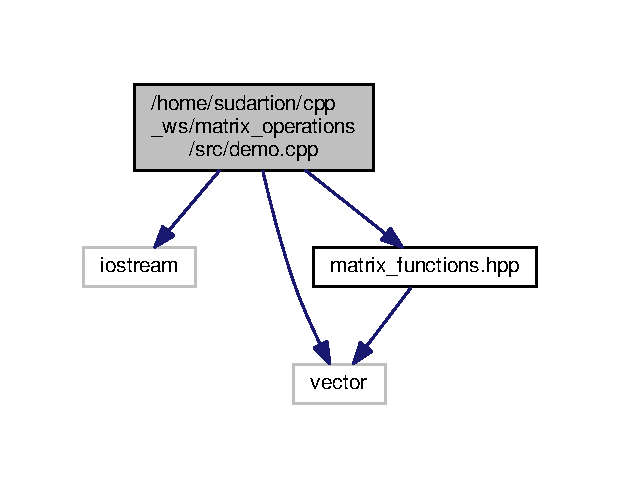
\includegraphics[width=298pt]{demo_8cpp__incl}
\end{center}
\end{figure}
\subsection*{Functions}
\begin{DoxyCompactItemize}
\item 
int {\bfseries main} ()\hypertarget{demo_8cpp_ae66f6b31b5ad750f1fe042a706a4e3d4}{}\label{demo_8cpp_ae66f6b31b5ad750f1fe042a706a4e3d4}

\end{DoxyCompactItemize}


\subsection{Detailed Description}
\hyperlink{classMatrix}{Matrix} operations definition. 

M\+IT License Copyright (c) 2018 Sudarshan Raghunathan Permission is hereby granted, free of charge, to any person obtaining a copy of this software and associated documentation files (the \char`\"{}\+Software\char`\"{}), to deal in the Software without restriction, including without limitation the rights to use, copy, modify, merge, publish, distribute, sublicense, and/or sell copies of the Software, and to permit persons to whom the Software is furnished to do so, subject to the following conditions\+: The above copyright notice and this permission notice shall be included in all copies or substantial portions of the Software. T\+HE S\+O\+F\+T\+W\+A\+RE IS P\+R\+O\+V\+I\+D\+ED \char`\"{}\+A\+S I\+S\char`\"{}, W\+I\+T\+H\+O\+UT W\+A\+R\+R\+A\+N\+TY OF A\+NY K\+I\+ND, E\+X\+P\+R\+E\+SS OR I\+M\+P\+L\+I\+ED, I\+N\+C\+L\+U\+D\+I\+NG B\+UT N\+OT L\+I\+M\+I\+T\+ED TO T\+HE W\+A\+R\+R\+A\+N\+T\+I\+ES OF M\+E\+R\+C\+H\+A\+N\+T\+A\+B\+I\+L\+I\+TY, F\+I\+T\+N\+E\+SS F\+OR A P\+A\+R\+T\+I\+C\+U\+L\+AR P\+U\+R\+P\+O\+SE A\+ND N\+O\+N\+I\+N\+F\+R\+I\+N\+G\+E\+M\+E\+NT. IN NO E\+V\+E\+NT S\+H\+A\+LL T\+HE A\+U\+T\+H\+O\+RS OR C\+O\+P\+Y\+R\+I\+G\+HT H\+O\+L\+D\+E\+RS BE L\+I\+A\+B\+LE F\+OR A\+NY C\+L\+A\+IM, D\+A\+M\+A\+G\+ES OR O\+T\+H\+ER L\+I\+A\+B\+I\+L\+I\+TY, W\+H\+E\+T\+H\+ER IN AN A\+C\+T\+I\+ON OF C\+O\+N\+T\+R\+A\+CT, T\+O\+RT OR O\+T\+H\+E\+R\+W\+I\+SE, A\+R\+I\+S\+I\+NG F\+R\+OM, O\+UT OF OR IN C\+O\+N\+N\+E\+C\+T\+I\+ON W\+I\+TH T\+HE S\+O\+F\+T\+W\+A\+RE OR T\+HE U\+SE OR O\+T\+H\+ER D\+E\+A\+L\+I\+N\+GS IN T\+HE S\+O\+F\+T\+W\+A\+RE.

\begin{DoxyCopyright}{Copyright}
Copyright 2018 Sudarshan Raghunathan
\end{DoxyCopyright}
\begin{DoxyAuthor}{Author}
Sudarshan Raghunathan 
\end{DoxyAuthor}

\hypertarget{main_8cpp}{}\section{/home/sudartion/cpp\+\_\+ws/matrix\+\_\+operations/test/main.cpp File Reference}
\label{main_8cpp}\index{/home/sudartion/cpp\+\_\+ws/matrix\+\_\+operations/test/main.\+cpp@{/home/sudartion/cpp\+\_\+ws/matrix\+\_\+operations/test/main.\+cpp}}


Test cases for code coverage.  


{\ttfamily \#include $<$gtest/gtest.\+h$>$}\\*
Include dependency graph for main.\+cpp\+:
\nopagebreak
\begin{figure}[H]
\begin{center}
\leavevmode
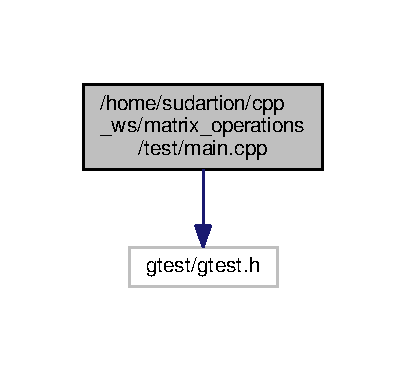
\includegraphics[width=195pt]{main_8cpp__incl}
\end{center}
\end{figure}
\subsection*{Functions}
\begin{DoxyCompactItemize}
\item 
int {\bfseries main} (int argc, char $\ast$argv\mbox{[}$\,$\mbox{]})\hypertarget{main_8cpp_a0ddf1224851353fc92bfbff6f499fa97}{}\label{main_8cpp_a0ddf1224851353fc92bfbff6f499fa97}

\end{DoxyCompactItemize}


\subsection{Detailed Description}
Test cases for code coverage. 

M\+IT License Copyright (c) 2018 Sudarshan Raghunathan Permission is hereby granted, free of charge, to any person obtaining a copy of this software and associated documentation files (the \char`\"{}\+Software\char`\"{}), to deal in the Software without restriction, including without limitation the rights to use, copy, modify, merge, publish, distribute, sublicense, and/or sell copies of the Software, and to permit persons to whom the Software is furnished to do so, subject to the following conditions\+: The above copyright notice and this permission notice shall be included in all copies or substantial portions of the Software. T\+HE S\+O\+F\+T\+W\+A\+RE IS P\+R\+O\+V\+I\+D\+ED \char`\"{}\+A\+S I\+S\char`\"{}, W\+I\+T\+H\+O\+UT W\+A\+R\+R\+A\+N\+TY OF A\+NY K\+I\+ND, E\+X\+P\+R\+E\+SS OR I\+M\+P\+L\+I\+ED, I\+N\+C\+L\+U\+D\+I\+NG B\+UT N\+OT L\+I\+M\+I\+T\+ED TO T\+HE W\+A\+R\+R\+A\+N\+T\+I\+ES OF M\+E\+R\+C\+H\+A\+N\+T\+A\+B\+I\+L\+I\+TY, F\+I\+T\+N\+E\+SS F\+OR A P\+A\+R\+T\+I\+C\+U\+L\+AR P\+U\+R\+P\+O\+SE A\+ND N\+O\+N\+I\+N\+F\+R\+I\+N\+G\+E\+M\+E\+NT. IN NO E\+V\+E\+NT S\+H\+A\+LL T\+HE A\+U\+T\+H\+O\+RS OR C\+O\+P\+Y\+R\+I\+G\+HT H\+O\+L\+D\+E\+RS BE L\+I\+A\+B\+LE F\+OR A\+NY C\+L\+A\+IM, D\+A\+M\+A\+G\+ES OR O\+T\+H\+ER L\+I\+A\+B\+I\+L\+I\+TY, W\+H\+E\+T\+H\+ER IN AN A\+C\+T\+I\+ON OF C\+O\+N\+T\+R\+A\+CT, T\+O\+RT OR O\+T\+H\+E\+R\+W\+I\+SE, A\+R\+I\+S\+I\+NG F\+R\+OM, O\+UT OF OR IN C\+O\+N\+N\+E\+C\+T\+I\+ON W\+I\+TH T\+HE S\+O\+F\+T\+W\+A\+RE OR T\+HE U\+SE OR O\+T\+H\+ER D\+E\+A\+L\+I\+N\+GS IN T\+HE S\+O\+F\+T\+W\+A\+RE.

\begin{DoxyCopyright}{Copyright}
Copyright 2018 Sudarshan Raghunathan
\end{DoxyCopyright}
\begin{DoxyAuthor}{Author}
Sudarshan Raghunathan 
\end{DoxyAuthor}

\hypertarget{test_8cpp}{}\section{/home/sudartion/cpp\+\_\+ws/matrix\+\_\+operations/test/test.cpp File Reference}
\label{test_8cpp}\index{/home/sudartion/cpp\+\_\+ws/matrix\+\_\+operations/test/test.\+cpp@{/home/sudartion/cpp\+\_\+ws/matrix\+\_\+operations/test/test.\+cpp}}


\hyperlink{classMatrix}{Matrix} operations definition.  


{\ttfamily \#include $<$gtest/gtest.\+h$>$}\\*
{\ttfamily \#include $<$iostream$>$}\\*
{\ttfamily \#include $<$vector$>$}\\*
{\ttfamily \#include $<$../include/matrix\+\_\+functions.\+hpp$>$}\\*
Include dependency graph for test.\+cpp\+:
\nopagebreak
\begin{figure}[H]
\begin{center}
\leavevmode
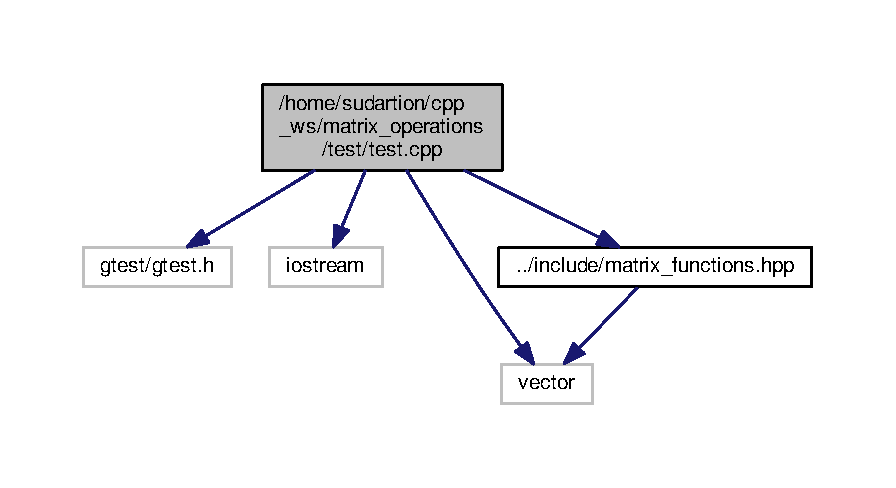
\includegraphics[width=350pt]{test_8cpp__incl}
\end{center}
\end{figure}
\subsection*{Functions}
\begin{DoxyCompactItemize}
\item 
int \hyperlink{test_8cpp_a5aaca9a11f445f56e6951e6844260950}{testing\+\_\+multiplication} ()
\begin{DoxyCompactList}\small\item\em Test function to verify the output matrix indices. \end{DoxyCompactList}\item 
bool \hyperlink{test_8cpp_a9c4346cef711daf44572e8f4abbe09ee}{testing\+\_\+multi\+\_\+index1} ()
\begin{DoxyCompactList}\small\item\em Test function to see if output of multiplication occurs only if two matrices have correct indices. \end{DoxyCompactList}\item 
bool \hyperlink{test_8cpp_a056b3b6d2dde6f6a2479791fa5be3354}{testing\+\_\+negindex} ()
\begin{DoxyCompactList}\small\item\em Test function to see if one of the indices are negative. \end{DoxyCompactList}\item 
bool \hyperlink{test_8cpp_a94f5d458d8941d68bc07bdab16fab022}{testing\+\_\+multi\+\_\+index} ()
\begin{DoxyCompactList}\small\item\em Test multiplication if indices are wrong. \end{DoxyCompactList}\item 
int \hyperlink{test_8cpp_a6eeed4efaf960ef0379845e7b899e7b9}{testing\+\_\+transpose} ()
\begin{DoxyCompactList}\small\item\em Function to test successful transpose. \end{DoxyCompactList}\item 
\hyperlink{test_8cpp_aea8c869db9e2b62fd63ed0c74b36ce1c}{T\+E\+ST} (Matrix\+Test, multiplication\+\_\+output\+\_\+index)\hypertarget{test_8cpp_aea8c869db9e2b62fd63ed0c74b36ce1c}{}\label{test_8cpp_aea8c869db9e2b62fd63ed0c74b36ce1c}

\begin{DoxyCompactList}\small\item\em Test case to ensure correct multiplication output. \end{DoxyCompactList}\item 
\hyperlink{test_8cpp_a7500f56b246d4a1e5f28799b4344a550}{T\+E\+ST} (Matrix\+Test, negative\+\_\+index\+\_\+check)\hypertarget{test_8cpp_a7500f56b246d4a1e5f28799b4344a550}{}\label{test_8cpp_a7500f56b246d4a1e5f28799b4344a550}

\begin{DoxyCompactList}\small\item\em Test case to check if any indices are negative. \end{DoxyCompactList}\item 
\hyperlink{test_8cpp_adf505bf7f9fe9a39997a0656e88c6b88}{T\+E\+ST} (Matrix\+Test, multiplication\+\_\+index\+\_\+check\+\_\+fail)\hypertarget{test_8cpp_adf505bf7f9fe9a39997a0656e88c6b88}{}\label{test_8cpp_adf505bf7f9fe9a39997a0656e88c6b88}

\begin{DoxyCompactList}\small\item\em Test case to ensure correct multiplication input. \end{DoxyCompactList}\item 
\hyperlink{test_8cpp_a492792847eedfbe94cf3c5c8e09c4e27}{T\+E\+ST} (Matrix\+Test, multiplication\+\_\+index\+\_\+check\+\_\+pass)\hypertarget{test_8cpp_a492792847eedfbe94cf3c5c8e09c4e27}{}\label{test_8cpp_a492792847eedfbe94cf3c5c8e09c4e27}

\begin{DoxyCompactList}\small\item\em Test case to see if it fails for bad multiplication inputs. \end{DoxyCompactList}\item 
\hyperlink{test_8cpp_a023db31462c939b777b96a48b3c1b181}{T\+E\+ST} (Matrix\+Test, transpose\+\_\+output\+\_\+test)\hypertarget{test_8cpp_a023db31462c939b777b96a48b3c1b181}{}\label{test_8cpp_a023db31462c939b777b96a48b3c1b181}

\begin{DoxyCompactList}\small\item\em Test case to ensure correct transposition. \end{DoxyCompactList}\end{DoxyCompactItemize}


\subsection{Detailed Description}
\hyperlink{classMatrix}{Matrix} operations definition. 

Test cases for code coverage.

M\+IT License Copyright (c) 2018 Sudarshan Raghunathan Permission is hereby granted, free of charge, to any person obtaining a copy of this software and associated documentation files (the \char`\"{}\+Software\char`\"{}), to deal in the Software without restriction, including without limitation the rights to use, copy, modify, merge, publish, distribute, sublicense, and/or sell copies of the Software, and to permit persons to whom the Software is furnished to do so, subject to the following conditions\+: The above copyright notice and this permission notice shall be included in all copies or substantial portions of the Software. T\+HE S\+O\+F\+T\+W\+A\+RE IS P\+R\+O\+V\+I\+D\+ED \char`\"{}\+A\+S I\+S\char`\"{}, W\+I\+T\+H\+O\+UT W\+A\+R\+R\+A\+N\+TY OF A\+NY K\+I\+ND, E\+X\+P\+R\+E\+SS OR I\+M\+P\+L\+I\+ED, I\+N\+C\+L\+U\+D\+I\+NG B\+UT N\+OT L\+I\+M\+I\+T\+ED TO T\+HE W\+A\+R\+R\+A\+N\+T\+I\+ES OF M\+E\+R\+C\+H\+A\+N\+T\+A\+B\+I\+L\+I\+TY, F\+I\+T\+N\+E\+SS F\+OR A P\+A\+R\+T\+I\+C\+U\+L\+AR P\+U\+R\+P\+O\+SE A\+ND N\+O\+N\+I\+N\+F\+R\+I\+N\+G\+E\+M\+E\+NT. IN NO E\+V\+E\+NT S\+H\+A\+LL T\+HE A\+U\+T\+H\+O\+RS OR C\+O\+P\+Y\+R\+I\+G\+HT H\+O\+L\+D\+E\+RS BE L\+I\+A\+B\+LE F\+OR A\+NY C\+L\+A\+IM, D\+A\+M\+A\+G\+ES OR O\+T\+H\+ER L\+I\+A\+B\+I\+L\+I\+TY, W\+H\+E\+T\+H\+ER IN AN A\+C\+T\+I\+ON OF C\+O\+N\+T\+R\+A\+CT, T\+O\+RT OR O\+T\+H\+E\+R\+W\+I\+SE, A\+R\+I\+S\+I\+NG F\+R\+OM, O\+UT OF OR IN C\+O\+N\+N\+E\+C\+T\+I\+ON W\+I\+TH T\+HE S\+O\+F\+T\+W\+A\+RE OR T\+HE U\+SE OR O\+T\+H\+ER D\+E\+A\+L\+I\+N\+GS IN T\+HE S\+O\+F\+T\+W\+A\+RE.

\begin{DoxyCopyright}{Copyright}
Copyright 2018 Sudarshan Raghunathan
\end{DoxyCopyright}
\begin{DoxyAuthor}{Author}
Sudarshan Raghunathans
\end{DoxyAuthor}
M\+IT License Copyright (c) 2018 Sudarshan Raghunathan Permission is hereby granted, free of charge, to any person obtaining a copy of this software and associated documentation files (the \char`\"{}\+Software\char`\"{}), to deal in the Software without restriction, including without limitation the rights to use, copy, modify, merge, publish, distribute, sublicense, and/or sell copies of the Software, and to permit persons to whom the Software is furnished to do so, subject to the following conditions\+: The above copyright notice and this permission notice shall be included in all copies or substantial portions of the Software. T\+HE S\+O\+F\+T\+W\+A\+RE IS P\+R\+O\+V\+I\+D\+ED \char`\"{}\+A\+S I\+S\char`\"{}, W\+I\+T\+H\+O\+UT W\+A\+R\+R\+A\+N\+TY OF A\+NY K\+I\+ND, E\+X\+P\+R\+E\+SS OR I\+M\+P\+L\+I\+ED, I\+N\+C\+L\+U\+D\+I\+NG B\+UT N\+OT L\+I\+M\+I\+T\+ED TO T\+HE W\+A\+R\+R\+A\+N\+T\+I\+ES OF M\+E\+R\+C\+H\+A\+N\+T\+A\+B\+I\+L\+I\+TY, F\+I\+T\+N\+E\+SS F\+OR A P\+A\+R\+T\+I\+C\+U\+L\+AR P\+U\+R\+P\+O\+SE A\+ND N\+O\+N\+I\+N\+F\+R\+I\+N\+G\+E\+M\+E\+NT. IN NO E\+V\+E\+NT S\+H\+A\+LL T\+HE A\+U\+T\+H\+O\+RS OR C\+O\+P\+Y\+R\+I\+G\+HT H\+O\+L\+D\+E\+RS BE L\+I\+A\+B\+LE F\+OR A\+NY C\+L\+A\+IM, D\+A\+M\+A\+G\+ES OR O\+T\+H\+ER L\+I\+A\+B\+I\+L\+I\+TY, W\+H\+E\+T\+H\+ER IN AN A\+C\+T\+I\+ON OF C\+O\+N\+T\+R\+A\+CT, T\+O\+RT OR O\+T\+H\+E\+R\+W\+I\+SE, A\+R\+I\+S\+I\+NG F\+R\+OM, O\+UT OF OR IN C\+O\+N\+N\+E\+C\+T\+I\+ON W\+I\+TH T\+HE S\+O\+F\+T\+W\+A\+RE OR T\+HE U\+SE OR O\+T\+H\+ER D\+E\+A\+L\+I\+N\+GS IN T\+HE S\+O\+F\+T\+W\+A\+RE.

\begin{DoxyCopyright}{Copyright}
Copyright 2018 Sudarshan Raghunathan
\end{DoxyCopyright}
\begin{DoxyAuthor}{Author}
Sudarshan Raghunathan 
\end{DoxyAuthor}


\subsection{Function Documentation}
\index{test.\+cpp@{test.\+cpp}!testing\+\_\+multi\+\_\+index@{testing\+\_\+multi\+\_\+index}}
\index{testing\+\_\+multi\+\_\+index@{testing\+\_\+multi\+\_\+index}!test.\+cpp@{test.\+cpp}}
\subsubsection[{\texorpdfstring{testing\+\_\+multi\+\_\+index()}{testing_multi_index()}}]{\setlength{\rightskip}{0pt plus 5cm}bool testing\+\_\+multi\+\_\+index (
\begin{DoxyParamCaption}
{}
\end{DoxyParamCaption}
)}\hypertarget{test_8cpp_a94f5d458d8941d68bc07bdab16fab022}{}\label{test_8cpp_a94f5d458d8941d68bc07bdab16fab022}


Test multiplication if indices are wrong. 

\begin{DoxyReturn}{Returns}
flag2 returns false when indices are wrong 
\end{DoxyReturn}
\index{test.\+cpp@{test.\+cpp}!testing\+\_\+multi\+\_\+index1@{testing\+\_\+multi\+\_\+index1}}
\index{testing\+\_\+multi\+\_\+index1@{testing\+\_\+multi\+\_\+index1}!test.\+cpp@{test.\+cpp}}
\subsubsection[{\texorpdfstring{testing\+\_\+multi\+\_\+index1()}{testing_multi_index1()}}]{\setlength{\rightskip}{0pt plus 5cm}bool testing\+\_\+multi\+\_\+index1 (
\begin{DoxyParamCaption}
{}
\end{DoxyParamCaption}
)}\hypertarget{test_8cpp_a9c4346cef711daf44572e8f4abbe09ee}{}\label{test_8cpp_a9c4346cef711daf44572e8f4abbe09ee}


Test function to see if output of multiplication occurs only if two matrices have correct indices. 

\begin{DoxyReturn}{Returns}
true if multiplication went successfully 
\end{DoxyReturn}
\index{test.\+cpp@{test.\+cpp}!testing\+\_\+multiplication@{testing\+\_\+multiplication}}
\index{testing\+\_\+multiplication@{testing\+\_\+multiplication}!test.\+cpp@{test.\+cpp}}
\subsubsection[{\texorpdfstring{testing\+\_\+multiplication()}{testing_multiplication()}}]{\setlength{\rightskip}{0pt plus 5cm}int testing\+\_\+multiplication (
\begin{DoxyParamCaption}
{}
\end{DoxyParamCaption}
)}\hypertarget{test_8cpp_a5aaca9a11f445f56e6951e6844260950}{}\label{test_8cpp_a5aaca9a11f445f56e6951e6844260950}


Test function to verify the output matrix indices. 

\begin{DoxyReturn}{Returns}
1 if multiplication went successfully 
\end{DoxyReturn}
\index{test.\+cpp@{test.\+cpp}!testing\+\_\+negindex@{testing\+\_\+negindex}}
\index{testing\+\_\+negindex@{testing\+\_\+negindex}!test.\+cpp@{test.\+cpp}}
\subsubsection[{\texorpdfstring{testing\+\_\+negindex()}{testing_negindex()}}]{\setlength{\rightskip}{0pt plus 5cm}bool testing\+\_\+negindex (
\begin{DoxyParamCaption}
{}
\end{DoxyParamCaption}
)}\hypertarget{test_8cpp_a056b3b6d2dde6f6a2479791fa5be3354}{}\label{test_8cpp_a056b3b6d2dde6f6a2479791fa5be3354}


Test function to see if one of the indices are negative. 

\begin{DoxyReturn}{Returns}
flag1 is false if one of the input indices is negative 
\end{DoxyReturn}
\index{test.\+cpp@{test.\+cpp}!testing\+\_\+transpose@{testing\+\_\+transpose}}
\index{testing\+\_\+transpose@{testing\+\_\+transpose}!test.\+cpp@{test.\+cpp}}
\subsubsection[{\texorpdfstring{testing\+\_\+transpose()}{testing_transpose()}}]{\setlength{\rightskip}{0pt plus 5cm}int testing\+\_\+transpose (
\begin{DoxyParamCaption}
{}
\end{DoxyParamCaption}
)}\hypertarget{test_8cpp_a6eeed4efaf960ef0379845e7b899e7b9}{}\label{test_8cpp_a6eeed4efaf960ef0379845e7b899e7b9}


Function to test successful transpose. 

\begin{DoxyReturn}{Returns}
1 if transpose is successful 
\end{DoxyReturn}

%--- End generated contents ---

% Index
\backmatter
\newpage
\phantomsection
\clearemptydoublepage
\addcontentsline{toc}{chapter}{Index}
\printindex

\end{document}
